\documentclass[runningheads]{llncs}

\usepackage[T1]{fontenc}
\usepackage{graphicx}
\usepackage{url}

\begin{document}

\title{Real-Time Online Auction Platform for High-Value Assets}

\author{
Doan Viet\inst{1}
\and
Le Hoang\inst{1}
\and
Tran Thanh Hung\inst{1}
\and
Nguyen Tien Quan\inst{1}
\and
Nguyen Huu Tai\inst{1}
}

\authorrunning{D. V.  et al.}

\institute{
FPT University, Da Nang City, Vietnam
}

\maketitle

\begin{abstract}

Online auctions have become increasingly popular due to the rapid growth of e-commerce and digital marketplaces. However, many existing auction systems face challenges related to real-time bid synchronization, scalability, and notification delivery under high user concurrency.

This paper presents a Real-Time Online Auction Platform designed for high-value assets such as collectibles, rare cards, antiques, and electronic devices.

The proposed platform adopts a microservices architecture to improve scalability and maintainability while utilizing WebSocket technology to provide low-latency bid updates. The system supports real-time bidding, auction room management, user authentication, payment processing, and instant notifications.

Furthermore, role-based access control enables administrators to monitor and manage auction activities effectively.

Experimental evaluation demonstrates that the platform can deliver real-time updates efficiently while maintaining system responsiveness during concurrent bidding sessions.

The proposed solution provides a practical foundation for developing modern online auction applications that require reliability, scalability, and fairness.

\keywords{Online Auction \and Real-Time Systems \and WebSocket \and Microservices \and E-Commerce}

\end{abstract}

%-------------------------------------------------------
\section{Introduction}

The rapid expansion of e-commerce has transformed traditional trading methods into digital platforms. Among these developments, online auction systems have emerged as an effective mechanism for buying and selling valuable assets through competitive bidding processes.

Despite their popularity, many existing auction platforms experience limitations in handling real-time bid updates, ensuring fair competition among participants, and maintaining system performance during periods of high traffic. Delayed bid synchronization may negatively affect user experience and reduce trust in the auction process.

To address these challenges, this paper proposes a Real-Time Online Auction Platform that leverages WebSocket communication and microservices architecture. The platform enables instant bid propagation, scalable service deployment, and efficient auction management.

The primary contributions of this study are as follows:

\begin{itemize}
\item Design of a scalable microservices-based auction architecture.
\item Development of a real-time bidding mechanism using WebSocket.
\item Implementation of notification services for auction events.
\item Integration of role-based administration and monitoring functions.
\end{itemize}

The remainder of this paper is organized as follows. Section 2 discusses related work. Section 3 presents the proposed methodology. Section 4 describes implementation details. Section 5 discusses results and evaluation. Finally, Section 6 concludes the paper and suggests future work.

%-------------------------------------------------------
\section{Related Work}

\subsection{Online Auction Systems}

Online auction platforms have been extensively studied within the e-commerce domain. Previous research has focused on bidding strategies, auction fairness, user trust, and transaction security. Commercial platforms such as eBay have demonstrated the feasibility of large-scale online auctions; however, real-time responsiveness remains a critical challenge \cite{ebay}.

\subsection{Real-Time Communication Technologies}

Traditional web applications commonly rely on HTTP request-response communication. However, technologies such as WebSocket provide full-duplex communication channels that enable servers to push updates to connected clients instantly\cite{websocket}. This significantly reduces latency and improves responsiveness in real-time applications.

\subsection{Microservices Architecture}

Microservices architecture decomposes applications into independently deployable services \cite{microservice}. Compared with monolithic systems, microservices improve scalability, maintainability, and fault isolation \cite{newman2021}. Consequently, many modern distributed systems adopt microservices to support large user populations and dynamic workloads.

\subsection{Research Gap}

Although previous studies have explored online auctions and real-time communication separately, limited research has focused on integrating WebSocket-based bidding mechanisms with microservices architecture for high-value asset auctions. This work aims to bridge that gap by proposing a comprehensive platform architecture.

%-------------------------------------------------------
\section{Methodology}

\subsection{System Architecture}

The proposed platform is organized into three major subsystems that support auction management and real-time bidding operations.

\begin{itemize}
\item Auction Customer Site
\item Auction Admin Site
\item Auction Real-Time Hub
\end{itemize}

The Auction Customer Site provides interfaces for bidders to browse auctions, join auction rooms, and place bids. The Auction Admin Site enables auction managers and administrators to create auctions, manage users, and monitor system activities.

The Auction Real-Time Hub is responsible for synchronizing bidding information among connected users through WebSocket communication. This component ensures that all participants receive instant updates whenever a new bid is submitted.

Figure~\ref{fig:architecture} illustrates the overall system architecture.

\begin{figure}[ht]
\centering
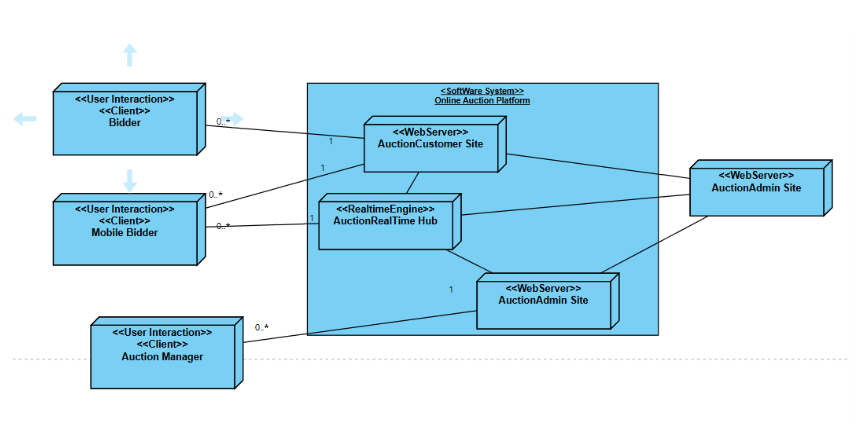
\includegraphics[width=\textwidth]{images/image_2026-06-16_193445989.png}
\caption{Overall System Architecture}
\label{fig:architecture}
\end{figure}

\subsection{Auction Workflow}

The auction process consists of the following steps:

\begin{enumerate}
\item User joins an auction room.
\item User submits a bid.
\item Bid Service validates the bid value.
\item Auction Service updates the highest bid.
\item Notification Service broadcasts updates to participants.
\item The system determines the winner when the auction ends.
\end{enumerate}

\subsection{Database Design}

The platform database contains the following core entities:

\begin{itemize}
\item User
\item AuctionRoom
\item AuctionItem
\item Bid
\item Payment
\item Notification
\end{itemize}

These entities collectively support auction management, bidding history tracking, payment processing, and user communication.

\subsection{Real-Time Bidding Mechanism}

WebSocket technology is employed to maintain persistent communication channels between clients and the server. Whenever a new bid is accepted, the server immediately broadcasts the updated auction status to all participants within the corresponding auction room.

This approach minimizes communication latency and ensures that all users receive synchronized auction information in real time.

%-------------------------------------------------------
\section{System Implementation}

The system is implemented using modern web technologies.

\begin{table}[ht]
\caption{Technology Stack}
\centering
\begin{tabular}{|l|l|}
\hline
Component & Technology \\ \hline
Frontend & ReactJS \\
Backend & Spring Boot \\
Database & PostgreSQL \\
Communication & WebSocket \\
Authentication & JWT \\
Containerization & Docker \\
\hline
\end{tabular}
\end{table}
JWT is adopted for stateless authentication and authorization in the proposed platform \cite{jwt}.
%-------------------------------------------------------
\section{Results and Discussion}

Functional testing was conducted to verify the correctness of the implemented features.

\begin{table}[ht]
\caption{Functional Testing Results}
\centering
\begin{tabular}{|l|l|}
\hline
Function & Result \\ \hline
User Login & Pass \\
Auction Creation & Pass \\
Join Auction Room & Pass \\
Place Bid & Pass \\
Real-Time Notification & Pass \\
Payment Processing & Pass \\
\hline
\end{tabular}
\end{table}

The results indicate that the proposed platform successfully supports real-time bidding and auction management while maintaining acceptable responsiveness under concurrent usage scenarios.

%-------------------------------------------------------
\section{Conclusion}

This paper presented a Real-Time Online Auction Platform for high-value assets. By integrating WebSocket technology with a microservices architecture, the platform provides real-time bidding capabilities, efficient auction management, and scalable deployment.

Future work will focus on integrating AI-based fraud detection, recommendation systems, and advanced analytics to further enhance platform performance and user experience.

%-------------------------------------------------------
\begin{thebibliography}{10}

\bibitem{newman2021}
Newman, S.:
Building Microservices.
O'Reilly Media (2021)

\bibitem{websocket}
Fette, I., Melnikov, A.:
The WebSocket Protocol.
RFC 6455 (2011)

\bibitem{microservice}
Dragoni, N., et al.:
Microservices: Yesterday, Today, and Tomorrow.
Springer International Publishing (2017)

\bibitem{ebay}
Kambil, A., van Heck, E.:
Making Markets: How Firms Can Design and Profit from Online Auctions and Exchanges.
Harvard Business School Press (2002)

\bibitem{jwt}
Jones, M., Bradley, J., Sakimura, N.:
JSON Web Token (JWT).
RFC 7519 (2015)

\end{thebibliography}

\end{document}